% Chapter - Player Study - Physical Health effects
\chapter{Physical Health Effects}
\label{chapter:player-study-physical}
\lhead{Chapter \ref{chapter:player-study-physical}. \emph{Player Study - Physical Health Effects}}

This chapter examines the survey results in the context of determining th game's effect on the physical health of its players. The questions in Table \ref{tbl:rg2-survey-questions} and their answers are the main focus of this chapter, but relevant answers to other questions are also included.

\section{Results for Change in Physical Activity}

This section presents the results for the player survey questions related to Research Questions \ref{RQ2.1}, \ref{RQ2.2} and \ref{RQ2.3}. A total of 2193 subjects responded to the questions \emph{"In an average week, how much time did you spend on physical activities (e.g. walking, running or biking) before you started playing Pokémon Go?"} and \emph{"In an average week, how much time do you spend on physical activities since you started playing Pokémon Go?"}. Table \ref{tbl:physical-activity-before-and-after} shows the number of responses to each question (column 2 and 3 respectively), as well as the change \todo{(should it say delta?)}, within each time category. Percentages for the \emph{Before} and \emph{After} columns are the percentage of total respondents for the respective category, while the percentage in the \emph{Change} column shows the relative increase or decrease (negative percentages) for that category. Note that the percentages are rounded to the closest integer, and due to rounding errors, the percentages in column 2 and 3 sum to 101 \% and 99 \% respectively.

\begin{table}[h]
	\centering
	\caption{Physical activity before and after Pokémon GO}
	\label{tbl:physical-activity-before-and-after}
	\begin{tabular}{|l|c|c|c|}
		\hline
		\textbf{Hours of activity} & \textbf{Before} & \textbf{After} & \textbf{Change} \\\hline\hline
		30 minutes or less	& 395 & 32 & -363\\
							& 18\% & 1\% & -92\%\\\hline
		An hour or less & 324 & 107 & -217\\
						& 15\% & 5\% & -67\%\\\hline
		2 hours or less & 384 & 268 & -116\\
						& 18\% & 12\% & -30\%\\\hline
		4 hours or less & 477 & 515 & 38\\
						& 22\% & 23\% & 8\%\\\hline
		8 hours or less & 394 & 566 & 172\\
						& 18\% & 26\% & 44\%\\\hline
		12 hours or less	& 132 & 365 & 233\\
							& 6\% & 17\% & 177\%\\\hline
		20 hours or less	& 61 & 206 & 145\\
							& 3\% & 9\% & 238\%\\\hline
		More than 20 hours	& 26 & 134 & 108\\
							& 1\% & 6\% & 415\%\\\hline
	\end{tabular}
\end{table}

Where Table \ref{tbl:physical-activity-before-and-after} showed the number of respondents in each time range before and after Pokémon GO, Table \ref{tbl:physical-activity-changed-category} shows the number and portion of respondents who remained in their category, went up one or more categories, or down one or more categories. This is a good indicator of how many respondents became more or less physically active, but will not be exact as some players became more active within the same range while others became less active within the same range. \todo{Should this paragraph and table be in analysis?}

\begin{table}[h]
	\centering
	\caption{How many respondents changed physical activity categories?}
	\label{tbl:physical-activity-changed-category}
	\begin{tabular}{|l|c|c|c|}
		\hline
		\textbf{Initial category} & \textbf{Increased} & \textbf{Stable} & \textbf{Decreased}\\
		\hline\hline
		30 minutes or less	& 372	& 23	& n/a\\
		& 94\%	& 6\%	& \\\hline
		An hour or less		& 276	& 44	& 4\\
		& 85\%	& 14\%	& 1\%\\\hline
		2 hours or less		& 321	& 44	& 6\\
		& 84\%	& 15\%	& 1\%\\\hline
		4 hours or less		& 332	& 136	& 9\\
		& 70\%	& 28\%	& 2\%\\\hline
		8 hours or less		& 220	& 166	& 8\\
		& 56\%	& 42\%	& 2\%\\\hline
		12 hours or less	& 59	& 65	& 8\\
		& 45\%	& 49\%	& 6\%\\\hline
		20 hours or less	& 25	& 32	& 4\\
		& 41\%	& 52\%	& 7\%\\\hline
		More than 20 hours	& n/a		& 23	& 3\\
		&	& 88\%	& 12\%\\\hline
		\hline
		Total				& 1605	& 546	& 42\\
		& 73\%	& 25\%	& 2\%\\\hline
	\end{tabular}
\end{table}

Figure \ref{fig:change-in-physical-activity} shows the change in physical activity relative to previous activity. The X-axis show weekly physical activity before Pokémon GO, while the Y-axis shows weekly physical activity after they started playing Pokémon GO, with both axes ranging from \emph{Less than 30 minutes} to \emph{More than 20 hours}. The green cells are players who increased their physical activity, while red cells are players who became less physically active after they started playing. Darker shades signify a larger difference, while the white cells indicate no change. \todo{Should this paragraph and figure be in analysis?}

\begin{figure}[h]
	\centering
	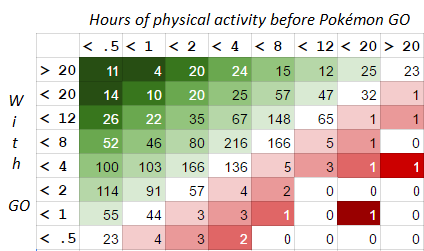
\includegraphics{Figures/change-in-physical-activity-table-colors}
	\caption{Change in physical activity with Pokémon GO}
	\label{fig:change-in-physical-activity}
\end{figure}

Respondents were also asked what activities lead to the increase in their physical activity, if they had become more physically active. Table \ref{tbl:physical-activity-sources} shows the number of respondents for each option out of 1823 respondents who reported an increase in physical activity.

\begin{table}[h]
	\centering
	\caption{Reasons for increased physical activity from Pokémon GO}
	\label{tbl:physical-activity-sources}
	\begin{tabular}{|c|c|c|c|}
		\hline
		\textbf{Detours} & \textbf{Errands} & \textbf{Pokéhunting} & \textbf{Other}\\\hline\hline
		1136 & 636 & 1576 & 89\\
		62\% & 35\% & 86\% & 5\%\\\hline
	\end{tabular}
\end{table}

It should be noted that 31 of these respondents (less than 2 \%) also chose the \emph{Not applicable} option, but it is uncertain what the implication of this is, given that they also selected other options. 25 of these 31 chose the same category for activity before and after, but because they are ranges it is still possible that they have increased activity within that range. The 6 remaining of those 31 reported more physical activity after Pokémon GO than before, so we can safely ignore the \emph{Not applicable} choice in their case. \todo{Should this be in Section \ref{sec:problems-with-survey} instead?}

The three categories \emph{Detours}, \emph{Errands} and \emph{Pokéhunting} were further explained in the question's options, see Appendix \ref{appendix:survey} \todo{(so I assume I don't have to repeat them here? Or should I?)}. Common examples of other activities leading to an increase in physical activity were players with dogs who walked them longer and more frequently to get in more play time or distance for their eggs, players who would walk during their breaks at work instead of sitting down, and players who went for longer or more frequent runs than previously. Many players who knew they should be going for walks but previously would not have, used Pokémon GO as a motivation to get outside and move around. Others found they enjoyed moving more and were motivated to start more rigorous exercise, while some even learned how to ride a bicycle so they could play more efficiently. \todo{Should I mention the respondents who said they increased physical activity for reasons unrelated to Pokémon GO? If so, here or in Section \ref{sec:problems-with-survey}?}

\todo{Mention 1) methods of transportation during play and 2) kilometers "walked" in the game? If so, here?}

\section{Analysis of Results for Change in Physical Activity}

The results were overwhelmingly positive. As seen in Table \ref{tbl:physical-activity-changed-category}, 73 \%, nearly three out of every four respondents, increased their physical activity enough to move up at least one category in physical activity after Pokémon GO compared to before. Table \ref{tbl:physical-activity-increased-multiple-categories} shows how many respondents from each initial category moved 2, 3, 4, 5 or 6 categories. Table \ref{tbl:physical-activity-average-categories-increased} shows how many categories players on average increased depending on their initial category. The \emph{Only increased} category shows the average increase for those who did in fact increase physical activity, while \emph{All} shows the numbers for all respondents who started within the respective category, including those who remained stable and those who decreased physical activity. \todo{Should these tables be moved to results?}

\begin{table}[h]
	\centering
	\caption{How many respondents increased physical activity by multiple categories?}
	\label{tbl:physical-activity-increased-multiple-categories}
	\begin{tabular}{|l|c|c|c|c|c|}
		\hline
		\textbf{Initial category} & \textbf{\( \geq2 \)} & \textbf{\( \geq3 \)} & \textbf{\( \geq4 \)}	& \textbf{\( \geq5 \)} & \textbf{\( \geq6 \)}\\
		\hline\hline
		30 minutes or less	& 317	& 203	& 103	& 51	& 25\\
							& 80\%	& 51\%	& 26\%	& 13\%	& 6\%\\\hline
		An hour or less		& 185	& 82	& 36	& 14	& 4\\
							& 57\%	& 25\%	& 11\%	& 4\%	& 1\%\\\hline
		2 hours or less		& 155	& 75	& 40	& 20	& n/a\\
							& 40\%	& 20\%	& 10\%	& 5\%	&\\\hline
		4 hours or less		& 116	& 49	& 24	& n/a	& n/a\\
							& 24\%	& 10\%	& 5\%	&		&\\\hline
		8 hours or less		& 72	& 15	& n/a	& n/a	& n/a\\
							& 18\%	& 4\%	& 		&		&\\\hline
		12 hours or less	& 12	& n/a	& n/a	& n/a	& n/a\\
							& 9\%	& 		&		&		&\\\hline
		\hline
		Total				& 857	& 424	& 203	& 85	& 29\\
							& 39\%	& 19\%	& 9\%	& 4\%	& 1\%\\\hline
	\end{tabular}
\end{table}

\begin{table}[h]
	\centering
	\caption{How many categories on average did players increase physical activity?}
	\label{tbl:physical-activity-average-categories-increased}
	\begin{tabular}{|l|c|c|}
		\hline
		\textbf{Initial category} & \textbf{Only increased} & \textbf{All}\\
		\hline\hline
		30 minutes or less	& 2.91	& 2.74\\
		An hour or less		& 2.16	& 1.83\\
		2 hours or less		& 1.90	& 1.57\\
		4 hours or less		& 1.57	& 1.06\\
		8 hours or less		& 1.40	& 0.75\\
		12 hours or less	& 1.20	& 0.45\\
		20 hours or less	& 1.00	& 0.23\\
		More than 20 hours	& n/a	& -0.27\\
		\hline
		Total				& 2.00	& 1.43\\\hline
	\end{tabular}
\end{table}

Because more than 92 \% of our respondents are adults by the WHO's definition of adults being aged 18-16, we are going to focus on the recommendations for adults. As discussed in Section \ref{sec:lit-study-physical-activity}, the WHO recommends that adults do at least 150 minutes of moderate-intensity physical activity per week. Using this recommendation, we categorize the players who are physically active less than this (the lower three categories) as \emph{Low activity} players. Respondents within the \emph{4 hours or less} and \emph{8 hours or less} categories will be categorized as \emph{Moderate activity} players, while the three remaining categories are \emph{High activity} players.

\begin{table}
	\centering
	\caption{Low/moderate/high activity players}
	\label{tbl:physical-activity-low-moderate-high}
	\begin{tabular}{|l|c|c|c|c|}
		\hline
		\textbf{Activity level}	& \textbf{Before}	& \textbf{After}	& \textbf{Change}	& \textbf{Categories increased}\\
		\hline\hline
		Low		& 1103	& 407	& -696	& 2.06\\
				& 50\%	& 19\%	& -63\%	&\\\hline
		Moderate& 871	& 1081	& 210	& 0.92\\
				& 40\%	& 49\%	& 24\%	&\\\hline
		High	& 219	& 705	& 486	& 0.31\\
				& 10\%	& 32\%	& 222\%	&\\\hline
	\end{tabular}
\end{table}

We see that while 50 \% of respondents were of low activity before Pokémon GO, this group only consisted of 19 \% of the respondents after Pokémon GO, a decrease of over 60 \%. The effect was larger for the lower activity ranges, where the number of respondents who had previously been active 30 minutes or less per week decreased by 92 \%, while the number who had previously been active between 1 and 2 hours per week only decreased by 30 \%. This is partly because the \emph{2 hours or less} category also saw an influx of players from the lower categories, but also because the lower ranges were narrower and thus easier to transcend. However, from Table \ref{tbl:physical-activity-average-categories-increased} we see that more than 50 \% of the respondents from the \emph{30 minutes or less} category increased their activity to a moderate level by jumping 3 or more categories, with the average number of categories increased for respondents initially placed in this category was 2.74.

The number of moderate activity players increased by 24 \%, which does not seem like a huge increase. However, paired with the fact that the number of high activity players more than tripled with a 222 \% increase, the number becomes more impressive, as this means the moderate activity category also "lost" quite a few of the players originally in this category. Respondents in the moderate activity category increased activity by a little less than one category on average. While this is not an enormous shift for these players, it places them safely within the range of the WHO's recommended weekly activity.

High activity players increased activity by 0.31 categories on average, with the majority of these increases coming from the players who had initially been active 12 hours or less. The initial members of the \emph{More than 20 hours} category decreased by 0.27 categories on average. The sample size was very small, however, consisting of only 26 respondents initially. The 0.27 category decrease is the result of three individuals and does not take into account that those in the \emph{More than 20 hours} category were unable to increase in category and that there were some respondents who mentioned in comments that they had in fact increased activity by 5-10 hours. It is however plausible that balancing a high physical activity week with playing Pokémon GO can be difficult, resulting in a slight decrease in physical activity from participating in game activities such as "camping" lures or nests. \todo{More on low-movement activities such as "camping".}

\todo{Althoff et al. ("Influence of Pokémon Go on Physical Activity ...") is highly relevant here and probably has some}

From Table \ref{tbl:physical-activity-sources}, we see that 62 \% of respondents listed \emph{Detours} as a cause for increased physical activity, while 86 \% listed \emph{Pokéhunting}. If and when a player stops playing Pokémon GO, they will no longer go out with the primary goal of catching or playing Pokémon. It is also unlikely that they will take detours when there is no goal with the detour other than taking it for the added activity. This unfortunately means that an increase in physical activity that originated from these sources is likely to revert should these players give up the game. 35 \% of respondents said they had started walking, biking \todo{(is "biking" too informal?)} or similar when performing errands or other day-to-day activities where they would previously have used some other mode of transportation such as a car. If these players stop playing the game, they could feasibly keep up this new routine, having realized it's not only possible to perform the activities without a car, but it also feels better to stay active, though it is unlikely to be the case for all of these players. For some members of the low activity category, being physically active more than before helped them realize they felt better with some physical activity in their routine, and some of these players started exercising outside of this. \todo{Check back on this paragraph later. Also needs to mention the follow-up results}

\todo{Only 19 \% left in low activity! Maybe in discussion/reflection/conclusion?}


\section{Results for Weight Loss, Feeling Healthier and Skipping Unhealthy Activities}

This section presents the results for the player survey questions related to Research Questions \ref{RQ2.4} and \ref{RQ2.5}. Table \ref{tbl:lost-weight-or-feeling-healthier} shows the categorized responses of 1478 respondents to the question \emph{Have you lost weight or in other ways feel more healthy than before you started playing Pokémon GO?}.

\begin{table}[h]
	\centering
	\caption{\emph{Have you lost weight or in other ways feel more healthy than before you started playing?} responses}
	\label{tbl:lost-weight-or-feeling-healthier}
	\begin{tabular}{|c|c|c|c|}
		\hline
		\textbf{Yes}	& \textbf{No}	& \textbf{N/A}	& \textbf{Unknown}\\
		\hline\hline
		738		& 671	& 19	& 50\\
		50\%	& 45\%	& 1\%	& 3\%\\\hline
	\end{tabular}
\end{table}

The \emph{No} respondents are players who did not experience any weight loss or improvement to health from playing the game. The \emph{Unknown} respondents did not know whether they had experienced any changes, and while some of them said \emph{"Probably"}, they have not been constrained to this category \todo{(is that necessary to mention?)}. The \emph{N/A} category are players who were already experiencing weight loss or changes to their health situation from other sources, such as diets, exercising or illnesses, prior to starting Pokémon GO. Their weight or health improvement progress continued while playing, but is assumed to be unrelated to Pokémon GO as the improvement had already started before they started playing, and these respondents were adamant that playing had not had an effect.

The \emph{Yes} category are the respondents who reported either weight loss or an improvement to one or more areas of their health. Out of these 738 respondents, 155 (21 \%) reported that they had lost weight. Other respondents reported a loss in body fat and/or gain in muscle mass while remaining at the same weight, while some noted a decrease in pant size while being unsure about changes to their weight. The most commonly reported improvement besides weight loss and generally feeling healthier was improved stamina or endurance, being able to walk or run faster, further and longer than before. Other improvements reported include eating and drinking better (drinking more water to stay hydrated and being less inclined to eat junk food), gain of motivation to exercise more, better sleep, less stress, easier breathing and feeling more alert. Some players reported that playing had helped them quit smoking, while a few lowered their blood pressure, experienced a positive effect on illnesses such as anemia, or an improved effect from their medication. Some players also used this question to note an improvement to mental health or happiness, which will be discussed further in Chapter \ref{chapter:player-study-mental}.

Players were also asked whether they had skipped any unhealthy activities in favor of playing Pokémon GO. Table \ref{tbl:skipping-unhealthy-activities} shows the 1629 responses to this question.

\begin{table}[h]
	\centering
	\caption{\emph{Have you skipped out on less healthy activities that you otherwise would have engaged in due to playing Pokémon Go instead?} responses}
	\label{tbl:skipping-unhealthy-activities}
	\begin{tabular}{|c|c|c|c|c|}
		\hline
		\textbf{Yes} & \textbf{No} & \textbf{Both} & \textbf{Opposite} & \textbf{N/A}\\
		\hline\hline
		415		& 1160	& 4		& 20	& 30\\
		25\%	& 71\%	& 0.25\%& 1\%	& 2\%\\\hline
	\end{tabular}
\end{table}

The \emph{No} category did not skip any activities they deemed unhealthy in favor of playing Pokémon GO, while the \emph{Yes} category did. The \emph{Both} category did less of one or more unhealthy activity, but more of another \todo{(too small to include? If so, which category to merge into, or just ignore?)}. The \emph{Opposite} category not only did not skip any unhealthy activities, but participated in more unhealthy activities because of the game than they would have without \todo{(merge into No-category and just mention these examples?)}. The \emph{N/A} category said they did not participate in any unhealthy activities neither before or after Pokémon GO.

\section{Analysis of Results for Weight Loss, Feeling Healthier and Skipping Unhealthy Activities}

While certainly not all individuals need to lose weight, the WHO reported that 39 \% of adults worldwide were overweight in 2014 \todo{[insert citation]}, while the NIDDK reported that more than 2 out of every 3 adults in the United States were overweight \todo{[insert citation]}. Therefore we can assume that the fact that over 10 \% of respondents lost weight is a positive thing overall. Out of the 84 subjects who responded with the amount of weight they had lost, the average respondent had lost just over 5.2 kg, ranging from 0.5 to 18.5 kg. However, not knowing the initial weight of these respondents, it is difficult to determine exactly how positive this is, as discussed in \ref{sec:problems-with-survey}.

There are a few other points to note regarding the weight loss data. Some players categorized as \emph{Yes}-respondents started diets or more focused exercise after they started playing Pokémon GO, meaning it is difficult to determine the impact of playing Pokémon GO in their weight loss. However, for many or most of these respondents, the lifestyle change was inspired by the increased activity and health improvements already experienced from playing Pokémon GO.

Others who lost weight were already underweight and actually needed to gain weight. While their loss of weight was not positive, most of these players also experienced a positive effect such as improvements to mental health, or help with physical conditions such as anemia.

Some of the \emph{No} players not only did not experience an improvement, but worsened their current state by exercising less or adopting bad habits such as eating more junk food or going to bars drinking when they otherwise would not have done so. These are mostly the same players as represented by the \emph{Opposite} category in Table \ref{tbl:skipping-unhealthy-activities}, although there are some players that do not overlap.

As seen in Table \ref{tbl:skipping-unhealthy-activities}, 25 \% of respondents said that they skipped unhealthy activities in favor of playing Pokémon GO. While the activities in question for a lot of these players (roughly 38 \%) were primarily watching TV or playing video games at home, it's not unlikely that many of these activities would have included snacks that were not consumed while out playing. There were also quite a few (more than 26 \%) who went out to play Pokémon instead of going to bars or otherwise consume alcohol. Others cut down on junk food, and some stopped snacking and overeating in general. Some players even managed to stop smoking due to playing. There were unfortunately also some players who started drinking more because their local bars had good access to Pokéstops, so sitting at those bars with lures became a habit. \todo{Is this paragraph ok as is?}

There is nothing about Pokémon GO itself that causes the physical health benefits experienced by its players, which are all due to the lifestyle changes playing the game brought, primarily the increased physical activity. However, it managed to motivate many players to experience this increased physical activity without marketing as an exercise application, and 50 \% of respondents experienced a tangible effect on their physical health from doing what they thought of as simply playing a game. \todo{Perhaps move this paragraph to reflection on results?}


\section{Results for Neglect and Negative Behavior}

The players who started exercising less or drinking more are not the only negative side effects of playing Pokémon GO. This section presents the results for the player survey questions related to Research Question \ref{RQ2.6}. Players were asked whether they had neglected other important areas of their life due to playing Pokémon GO, and 220 players responded that they had neglected to eat, drink or sleep enough. Some of these players became dehydrated, while others had little energy because of the lack of sleep. Three respondents neglected giving their feet the rest they needed and experienced serious problems because of this, where two developed tendinitis and one made a chronic condition worse. Some players were not used to spending large amounts of time outside during summer and experienced sunburns of varying severity.

Players were also asked whether they had trespassed, put themselves or others in dangerous situations or gotten into accidents. Almost 15 \% of the respondents had trespassed at least once, with 47 \% of them doing so knowingly. While trespassing often is uneventful and without significant risk, it has the potential to be dangerous in addition to being inconsiderate. 238 players, a little less than 11 \% of all the respondents, said they had put either themselves or others in one or more dangerous situations, with 94 \% endangering themselves and 33 \% admitting to endangering others. 92 players had been in accidents because of the game, whereof 2 were accidents with serious injury or property damage.

Of the players who had either endangered themselves or others, or gotten into accidents, 231 respondents chose to elaborate on the events. Table \ref{tbl:danger-or-accidents-elaboration} shows the most common causes for accidents and sources of endangerment.

\begin{table}[h]
	\centering
	\caption{\emph{If you have put yourself or others in dangerous situations, or gotten into accidents, because of Pokémon Go, could you elaborate?} categorized responses}
	\label{tbl:danger-or-accidents-elaboration}
	\begin{tabular}{|c|c|c|c|c|c|}
		\hline
		Driving	& Surroundings	& Traffic	& Bicycle	& Alone at night	& Bad neighborhood\\
		\hline\hline
		90		& 38			& 36		& 28		& 15				& 8\\
		39\%	& 16\%			& 16\%		& 12\%		& 6\%				& 3\%\\\hline
		%		\textbf{Category} & \textbf{Endangered} & \textbf{Accident} & \textbf{Total}\\
		%		\hline\hline
		%		Car				& 84	& 7		& 90\\
		%						& 36\%	& 3\%	& 39\%\\\hline
		%		Surroundings	& 22	& 26	& 38\\
		%						& 9\%	& 11\%	& 16\%\\\hline
		%		Traffic			& 33	& 10	& 36\\
		%						& 14\%	& 4\%	& 16\%\\\hline
		%		Bicycle			& 17	& 16	& 28\\
		%						& 7\%	& 7\%	& 12\%\\\hline
		%		Alone at night	& 11	& 1	& 28\\
		%						& 7\%	& 7\%	& 12\%\\\hline
	\end{tabular}
\end{table}

The \emph{Driving} category respondents put themselves or others in danger by playing Pokémon GO while driving, or were in accidents with their car because they were playing Pokémon GO.

The \emph{Surroundings} category are respondents who were not paying attention to their surroundings while playing (mostly on foot), many of whom got into accidents because of it.

The \emph{Traffic} category are respondents who either did not pay sufficient attention when walking in or around traffic because they were playing Pokémon GO, or drivers who got into or narrowly avoided accidents because someone else was playing.

The \emph{Bicycle} category are players who were playing while riding a bicycle, exposing themselves to risk and/or getting into accidents because of it. Another 5 respondents reported similar experiences using other methods of transportation, such as skateboards or \emph{hovedboards} \todo{(include picture of a hoverboard?)}.

The \emph{Alone at night} category are respondents who put themselves at risk by walking outside alone at night when they usually would not have, while the \emph{Bad neighborhood} category are players who ventured into dangerous neighborhoods to play.

\section{Analysis of Results for Neglect and Negative Behavior}

Just as any other engaging activity, Pokémon GO caused some players (roughly 10 \% of the total respondents) to neglect sleep, eating enough or staying hydrated. While this is not a new phenomenon, the extra physical activity Pokémon GO players are exposed to compared to activities such as computer games means that staying hydrated is extra important, particularly in the summer heat. On the game's loading screen, it encourages players to be aware of their surroundings. This place could also be used to remind players to stay hydrated while playing and encourage players to drink enough water. Another possible option is making every few Pokéstops claimed give this same reminder and encouragement, possibly based on geographic location or the current season to avoid making players tired of these warnings when the weather is less warm and prone to cause dehydration.

The greater issue, however, are players who drive and play at the same time. It is widely known \todo{[cite WHO]} that using a mobile phone while driving greatly increases chances of accidents happening, yet many still do it. That almost 2 out of every 5 respondents who endangered themselves or others were doing so by playing while driving is a serious issue that Niantic did make an effort to fix by blocking the game with a warning whenever the player was detected to be moving too fast to be on foot, asking the player not to play while driving, as seen in Figure \ref{fig:do-not-play-and-drive}. Some of these players did not even seem to realize that they were endangering not only themselves, but also other innocent people with their actions, as shown by the difference in number of respondents who said they were playing while driving and the number who said they had put themselves or others in danger. Only 7 of these players (less than 8 \% of the drivers) were involved in accidents because of playing while driving, and all of them were minor accidents with slight damage to the car, but if any of these 90 players had been less lucky, their actions could have been fatal. \todo{(include picture of in-game warning here)}

\begin{figure}[h]
	\centering
	\caption{\emph{Do not play Pokémon GO while driving} in-game warning}
	\label{fig:do-not-play-and-drive}
\end{figure}

Bikers were not quite as lucky while playing, and 16 out of the 28 (or 57 \%) got into accidents where they either hurt themselves, their bike, or hit someone else. Most of these accidents were minor, but one player hit an unexpectedly high speed bump while not paying attention and ended up with a broken arm. These numbers, while a small sample size, indicate that playing Pokémon GO while biking is not a good combination. While a total of 575 players reported using a bicycle as a method of transportation while playing, it is unknown how many of these played actively while on the bike, and we will have to rely on the numbers for those who explicitly mentioned playing while biking. It is however possible that the portion of players who play while riding a bicycle is larger, as several retailers reported increased sales of phone holders for bicycles. This would imply that playing while biking is relatively safer than originally assumed, but players should still show caution.

As previously mentioned and seen in Figure \ref{fig:loading-screen-aware-of-surroundings}, the loading screen for the game encourages players to remain aware of their surroundings while playing, and with good reason. Of the players who did not pay attention to their surroundings around traffic, 10 (28 \%) were involved in accidents. These players wandered into the street without looking properly or walked too close to the edge of the sidewalk and got hit by cyclists or side mirrors of cars. That only ten of these players were involved in accidents, and that none of them had serious consequences, is likely thanks to a good dose of luck \todo{(too informal?)}, and similarly to those who play and drive, this could have gone much worse with less luck.

26 (68 \%) of the players who did not pay attention to their surroundings in general were involved in accidents. While this portion seems staggeringly high, based on general observation of players in the wild, a much larger percentage of players than the 38 who mentioned it were playing without paying particularly close attention to their surroundings. It is likely that the 38 players who mentioned it were the ones who were involved in accidents or near-accidents because of it, while the majority of the other players avoided this. The players in this category who were involved in accidents experienced events such as crashing into things (signs, lamp posts, parked cars, low balconies and similar), kicking things or misplacing their step. There were sprains, bruises and minor cuts, but no serious accidents.

\begin{figure}[h]
	\centering
	\caption{Game loading screen encouraging players to remain aware of their surroundings while playing}
	\label{fig:loading-screen-aware-of-surroundings}
\end{figure}

The players in the \emph{Alone at night} and \emph{Bad neighborhood} categories ventured out into the night to play Pokémon when or where they should not have, and without Pokémon would not either. For the most part, no harm came to them, with the exception of two players: one player was mugged \todo{[insert link to newspaper article about it?]} and another was shot after, but not hit. Still, the placement of Pokéstops and spawns can cause players to take unnecessary risks and venture into areas they should not be in. This is also the reason why some areas, such as airports, often have no spawns or Pokéstops. Another similar cause, if a little more innocent, is players who followed paths on the map that were not actually paths in reality, ending up in minor accidents such as those experienced by the players who were unaware of their surroundings.

The other serious accident respondents were involved in because of playing Pokémon GO was a player who experienced serious damage to his car because he had driven out to play Pokémon. He was not playing while driving, but had he not gone out to play, the damage would not have happened. Other players reported similar, if less severe events with flat tires and minor damages to their cars because they had brought their car out to play.


% Chapter
\chapter{Mental Health Effects}
\label{chapter:player-study-mental}
\lhead{Chapter \ref{chapter:player-study-mental}. \emph{Player Study - Mental Health Effects}}

This chapter examines the survey results in the context of determining th game's effect on the mental health of its players. The questions in Table \ref{tbl:rg3-survey-questions} and their answers are the main focus of this chapter, but relevant answers to other questions are also included.

\section{Results for Change in Social Activity}

This section presents the results for the player survey questions related to Research Questions \ref{RQ3.1} and \ref{RQ3.2}. A total of 2192 subjects responded to the questions \emph{"In an average week, during your spare time, how much time did you spend socializing with other people (in person, outside your home) before you started playing Pokémon Go?"} and \emph{"In an average week, during your spare time, how much time do you spend socializing with other people (in person, outside your home) since you started playing Pokémon Go?"}. Table \ref{tbl:social-activity-before-and-after} shows the number of responses to each question (column 2 and 3 respectively), as well as the change \todo{(should it say delta?)}, within each time category. Percentages for the \emph{Before} and \emph{After} columns are the percentage of total respondents for the respective category, while the percentage in the \emph{Change} column shows the relative increase or decrease (negative percentages) for that category. Note that the percentages are rounded to the closest integer, and due to rounding errors, the percentages in column 2 and 3 both sum to 99 \% \todo{(consider removing this and similar remarks and just mention it in problems with survey section)}. \todo{This paragraph is more or less a carbon copy of the corresponding section in physical health chapter. Is that ok?}

\begin{table}[h]
	\centering
	\caption{Social activity before and after Pokémon GO}
	\label{tbl:social-activity-before-and-after}
	\begin{tabular}{|l|c|c|c|}
		\hline
		\textbf{Hours of activity} & \textbf{Before} & \textbf{After} & \textbf{Change} \\\hline\hline
		30 minutes or less	& 245 & 138 & -107\\
		& 11\% & 6\% & -44\%\\\hline
		An hour or less & 220 & 155 & -65\\
		& 10\% & 7\% & -30\%\\\hline
		2 hours or less & 396 & 314 & -82\\
		& 18\% & 14\% & -21\%\\\hline
		4 hours or less & 499 & 492 & -7\\
		& 23\% & 22\% & -1\%\\\hline
		8 hours or less & 416 & 478 & 62\\
		& 19\% & 22\% & 15\%\\\hline
		12 hours or less	& 204 & 307 & 103\\
		& 9\% & 14\% & 50\%\\\hline
		20 hours or less	& 116 & 175 & 59\\
		& 5\% & 8\% & 51\%\\\hline
		More than 20 hours	& 96 & 133 & 37\\
		& 4\% & 6\% & 39\%\\\hline
	\end{tabular}
\end{table}

Where Table \ref{tbl:social-activity-before-and-after} shows how many respondents shows the changes within each time range of social activity, Table \ref{tbl:social-activity-change-or-stable} shows the number of respondents who became less socially active, more socially active or did not change their amount of social interaction.

\begin{table}[h]
	\centering
	\caption{How many respondents changed social activity time categories?}
	\label{tbl:social-activity-change-or-stable}
	\begin{tabular}{|c|c|c|}
		\hline
		\textbf{Decreased} & \textbf{Stable} & \textbf{Increased}\\\hline\hline
		74		& 1353		& 765\\
		3\%		& 62\%		& 35\%\\\hline
	\end{tabular}
\end{table}

\section{Analysis of Results for Change in Social Activity}

\section{Social Interaction}
\label{sub:mental-health-social}

\todo{Mention division of tasks (searching for nearby pokes, scoping out gyms, and transporter/player), and that players on different teams still can cooperate and be on good terms}

\section{Exercise}

\section{A Sense of Purpose}

\section{Disappointment}

\section{Negative Behavior and Adversarial Relationships}